In this section the problem of how to adjust the endpoint of a curve to properly
lie on the other curve will be discussed.

Per Kopf-Lischinski, a T-junction node will be the node that is common for three
adjacent splines. For one of the splines, this will be a smooth node. Using the
the shading/contour edges heuristic with an unspecified input image, we get the
following output:

\begin{figure}[H]
  \centering
  
\includegraphics[width=0.8\textwidth]{assets/shading-heuristic.pdf}
  \caption{The non-blue splines share a shading edge}
\end{figure}

Some splines got visually disconnected and created an undesired result. To fix
this issue we adjust the endpoint of the non-blue curves to properly lie on the
blue curve. The end result will be the following image:

\begin{figure}[H]
  \centering
  
\includegraphics[width=0.8\textwidth]{assets/shading-heuristic-fixed.pdf}
\end{figure}

Kopf-Lischinski paper don't document extensively how to ``adjust the endpoint of
a curve to properly lie on the other curve'' and you'll need to verify that the
algorithm documented here is correct based on the sample images provided in the
paper.

You may had learnt how to generate the splines in \hyperref[blogpart2]{part 2}.
And you know that if you change the position of a node, the midpoint between
this node and adjacent nodes will change. With the midpoint being changed, the
parts that previously were fitting together will visually disconnect or overlap.
Given that, we cannot simply adjust some node position without screwing up parts
of the curve that were previously correct using the poor and simple data
representation from the other steps.

We don't want to change the representation too, because this is exactly the type
of representation expected by the optimizer in the next steps. We can, however,
insert extra nodes without screwing up the previously correct parts of the curve
and if we take care to make some of them collinear, then they won't interfere
with the visual representation we got.

Combining the previous idea with the idea of subdivision from
\href{http://en.wikipedia.org/wiki/De_Casteljau's_algorithm}{De Casteljau's
algorithm} it's possible to adjust the ``endpoint'' of the non-blue curves to
properly lie on the blue curve. It's just a matter of finding the correct
positions.

\begin{figure}[H]
  \centering
  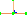
\includegraphics[width=0.8\textwidth]{assets/subdivision.pdf}
  \caption{\textbf{Splines} with control points highlighted with green circles}
\end{figure}

\begin{figure}[H]
  \centering
  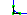
\includegraphics[width=0.8\textwidth]{assets/subdivision2.pdf}
  \caption{Blue \textbf{Bézier curve} with its points highlighted with green
    circles}
\end{figure}

After we subdivide a Bézier curve into two, there will be a new Bézier curve for
each other curve whose ``endpoint'' should properly lie on this curve. As such,
we only focus on one curve at each time. Now that we have the Bézier curve, we
need to compute the position of the new splines nodes exploring the
\emph{midpoint} feature. This process is represented in the next picture.

\begin{figure}[H]
  \centering
  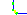
\includegraphics[width=0.8\textwidth]{assets/subdivision3.pdf}
  \caption{\textbf{Spline} with its control points highlighted with green
    circles. Yellow point is the point where the ``endpoint'' of the other
    curves should be placed.}
\end{figure}

The final result will have 5 points instead of one for a ``vertex'':

\begin{itemize}
\item The initial point to avoid screwing parts of the curve that previously
  were correct. Note that this point won't be visible, because it will be
  collinear with its neighbours points.
\item The new three points to properly adjust the ``endpoint'' of this curve.
  Note that extreme points (the first and the third) won't be visible, because
  they are collinear with its neighbour points.
\item The endpoint of the \textbf{Bézier curve}, then the two curves that are
  adjusted won't overlap. Note that this point is \textbf{not} smooth.
\end{itemize}

You may want to store this \emph{visibility} metadata for easily discard these
extra points when you convert the splines to Bézier curves in later steps.

This is the technique to ``adjust the endpoint of a curve to properly
lie on the other curve'', but this problem is not so easy, because (1) you'll
have to implement code to handle each node in the three splines and (2) the
position of nodes will also depend on the color similarity with neighbour
splines. The problem \#2 is exemplified in the image below (when compared to
previous examples):

\begin{figure}[H]
  \centering
  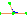
\includegraphics[width=0.8\textwidth]{assets/subdivision4.pdf}
  \caption{\textbf{Splines} with its control points highlighted with green
    circles.}
\end{figure}

Usually you will have to handle four different possibilities for \textbf{each}
of the five nodes. This means four large conditional branches. Nothing pleasant,
but you can reduce the code if you find the \emph{amount} that each condition
contributes to the final result.

You can find these conditions playing with experiments and boolean algebra or,
using a more elaborate approach, solving a simple linear system. This text won't
document all possible constants (at least not for this initial release) that you
can find, but you can check libdepixelize source code if you are in such a
hurry. This text will, however, give an example of how to solve a linear system
to find such constants.

These conditions are always related to connectivy among local nodes and will be
translated in expressions like ``is node X connected to its topleft node?''.

The constants $\frac{3}{16}$, $\frac{1}{16}$ and others happen a lot in this
problem. If you know a cool name for these constants, ping \emph{vinipsmaker}
and he will be happy to use your suggestion to name these constants.

\subsection{Solving the linear system}

Suppose that you have conditions \emph{A} and \emph{B} to determine the position
of the nodes, then you have four possibilities/branches to determine the
position of the nodes.

Suppose that, for the first node, you find the following positions for the
x-axis given the input conditions:

\begin{center}
  \begin{tabular}{|c|c|r|}
    \hline
    \textbf{\emph{A}} & \textbf{\emph{B}} & position \\
    \hline
    \emph{true} & \emph{true} & 0.0625 \\
    \emph{true} & \emph{false} & 0.09375 \\
    \emph{false} & \emph{true} & 0.09375 \\
    \emph{false} & \emph{false} & 0.125 \\
    \hline
  \end{tabular}
\end{center}

Now you can convert the previous table to a linear system replacing \emph{false}
by 0, \emph{true} by 1 and adding a column completely filled with ones for the
base value. For the previous table, this procedure will generate the following
augmented matrix:

$$\left(
  \begin{array}{ccc|r}
    1 & 1 & 1 & 0.0625 \\
    1 & 0 & 1 & 0.09375 \\
    0 & 1 & 1 & 0.09375 \\
    0 & 0 & 1 & 0.125
  \end{array}
\right)$$

After solve the system, you'll get the values $-\frac{1}{32}$, $-\frac{1}{32}$
and $\frac{1}{8}$ for $\chi_1$, $\chi_2$ and $\chi_3$, respectively. $\chi_3$ is
the base value, then the equation for the x position of the first node will be:

\begin{center}
  \texttt{node.pos.x} = $\frac{1}{8} - \text{\emph{A}} \frac{1}{32}
  - \text{\emph{B}} \frac{1}{32}$
\end{center}

Because $\chi_1$ and $\chi_2$ values are equal in this particular case, we can
reduce the formula:

\begin{center}
  \texttt{node.pos.x} = $\frac{1}{8} - (\text{\emph{A}}
  + \text{\emph{B}}) \frac{1}{32}$
\end{center}

That's it! Have fun finding the constants for each $x$ and $y$ for each node for
each ``adjust the endpoint of a curve to properly lie on the other curve''
procedure.
